\documentclass[a4paper,10pt]{article}
\usepackage{latexsym}
\usepackage{graphicx}
\usepackage{wrapfig}
\graphicspath{{./figuras/}}
\usepackage{subfigure}
\usepackage{multicol}
\usepackage{amsfonts}
\usepackage{amsmath}
\usepackage[utf8]{inputenc}
\usepackage[top=3cm, bottom=2.5cm, left=2.5cm, right=1cm]{geometry}


\title{MDF: Modelo de examen}
\author{{{\bf César I. Pairetti}}}

\newcommand{\mr}{\mathbb{R}}
\newcommand{\mn}{\mathbb{N}}
\newcommand{\mc}{\mathbb{C}}
\newcommand{\nti}{n \to \infty}
\newcommand{\mrn}{\mathbb{R}^n}
\newcommand{\iii}{\int_{-\infty}^{+\infty}}


\newcommand{\MDF}
{
\begin{center}
{\Large {\bf Ingeniería Mecánica:} Mecánica de los Fluidos}
\end{center}
\textit{Apellido, Nombre (Legajo)}: \hskip 8.cm Fecha:
\vspace{0.2cm}
}

\textwidth 16.cm

\begin{document}
\MDF
\noindent\underline{\textit{Segundo parcial}:} \textbf{Recuperatorio}
\begin{enumerate}
\item Se pretende analizar el campo de velocidades para el flujo laminar \textbf{desarrollado} en una cañería cilíndrica \textbf{infinita}, dado en la figura \ref{fig:hagen_poiseuille}. Considerando el problema \textbf{estacionario}:
\begin{enumerate}
  \item Defina las hipótesis para aplicar la ecuación de Navier-Stokes (\ref{eq:NSMom_u_cil}).
  \item Aplique simplificaciones por simetría y defina las condiciones de contorno matemáticamente.
  \item A partir de los tres apartados anteriores, obtenga la ecuación diferencial simplificada para el campo de velocidades.
  \item A partir de la solución, exprese el caudal circulante en función de los datos del problema.
\end{enumerate}

\begin{equation}\label{eq:NSMom_u_cil}
\begin{aligned}
\frac{1}{r}\frac{\partial }{\partial r} (r\,u_r)+ \frac{1}{r}\frac{\partial u_\theta}{\partial \theta} + \frac{\partial u_z}{\partial z}
&= 0 
\\
\frac{\partial u_z}{\partial t} + u_r\frac{\partial u_z}{\partial r} + \frac{u_\theta}{r}\frac{\partial u_z}{\partial \theta} + u_z \frac{\partial u_z}{\partial z}
&= -\frac{1}{\rho}\frac{\partial p}{\partial z}
+ \nu \left(\frac{1}{r}\frac{\partial}{\partial r}\left(r\frac{\partial u_z}{\partial r}\right) + \frac{1}{r^2}\frac{\partial^2 u_z}{\partial \theta^2} + \frac{\partial^2 u}{\partial z^2}\right)
\end{aligned}
\end{equation}
\begin{figure}[h!!]
\centering
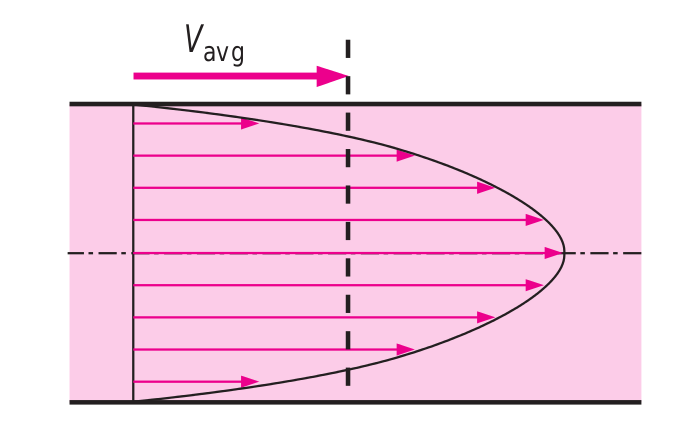
\includegraphics[width=0.35\textwidth]{hagen_poiseuille.png}
\caption{Flujo en un conducto cilíndrico}
\label{fig:hagen_poiseuille}
\end{figure}
%Pitot en auto
\item La figura \ref{fig:capa_limite} muestra la ubicación de un tubo de pitot en una superficie plana que se desplaza a una velocidad $U = 10$ km/h. Utilizando la solución de capa límite de Blasius, calcular la diferencia de presión que medirá el Pitot. Recuerde que la misma corresponde a la presión dinámica del flujo $p_{din} = \rho u^2/2$. A la distancia $L$, ¿cuál es el espesor de capa límite?

Una solución aproximada a la ecuación de Blasius es el polinomio de cuarto orden dado por la ecuación \ref{eq:PolBlasius}. A continuación se listan los datos del flujo:

\begin{figure}[h!!]
\centering
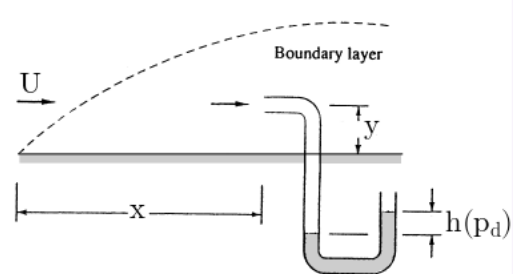
\includegraphics[width=0.5\textwidth]{capa_limite.png}
\caption{Pitot en placa plana, midiendo a una altura $h$}
\label{fig:capa_limite}
\end{figure}

$$\rho = 1.2 kg/m^3 \qquad \mu =1.75 \times 10^{-05} Pa s \qquad L = 0.1 m \qquad h = 0.001 m$$

\begin{equation}\label{eq:PolBlasius}
u/U = 0.0016217 \eta^4 - 0.0190921 \eta^3 + 0.0314731 \eta^2 + 0.3146989 \eta + 0.0015430 \qquad \qquad \eta = y \sqrt{\frac{U}{x\nu}}
%%  -9.2735e-05   1.5884e-03  -8.5280e-03   1.0741e-02  -8.2920e-03   3.3435e-01  -7.2436e-05 %% Mayor orden: 6
\end{equation}

\clearpage

%%Tobera convergente-divergente, sacado del Cimbala:
\item Entra aire a una tobera convergente-divergente, como se muestra en la figura \ref{fig:toberaConvDiv}, a $p_0 = 3$ MPa y $T_0 = 600$ K con velocidad despreciable. El flujo es estacionario, unidimensional e isentrópico con $k = 1.4$, $R^*= 287\;J/(K\,kg)$. Para obtener un Mach de salida $Ma_e = 2$, dada una garganta de área $A^* = 40 {cm}^2$, determinar:
\begin{enumerate}
\item Las condiciones de flujo en la garganta ($p_g$, $\rho_g$, $T_g$,$v_g$)
\item El flujo másico que circula por la tobera.
\item Las condiciones del flujo en el plano de la salida, inclusive el área de la salida de diseño ($p_s$, $\rho_s$, $T_s$,$v_s$).
\item En qué regiones de la tobera el flujo es sónico y en cuáles supersónico.
\end{enumerate}
\begin{figure}[h!!]
\centering
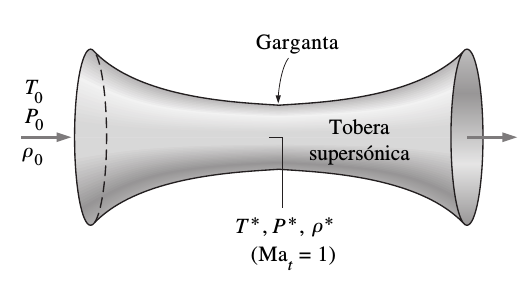
\includegraphics[width=0.6\textwidth]{toberaConvDiv.png}
%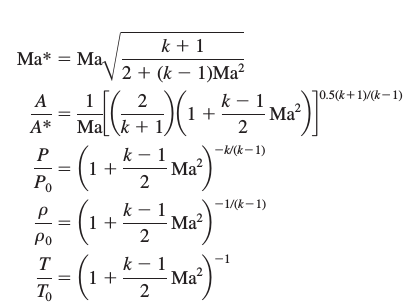
\includegraphics[width=0.6\textwidth]{eqs_comp.png}
%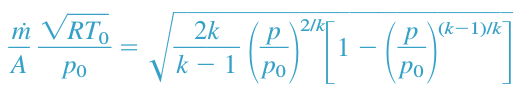
\includegraphics[width=0.5\textwidth]{mass_flux.png}
\caption{Tobera convergente divergente}
\label{fig:toberaConvDiv}
\end{figure}

\begin{equation*}
\begin{aligned}
\frac{A}{A^*} = \frac{1}{\text{Ma}}\left[\left(\frac{2}{k+1}\right) \left(1 + \frac{k-1}{2}\text{Ma}^2\right)\right]^{0.5(k+1)/(k-1)}
\qquad
\frac{T}{T_0} = \left(1 + \frac{k-1}{2}\text{Ma}^2\right)^{-1}
\\
\frac{p}{p_0} = \left(1 + \frac{k-1}{2}\text{Ma}^2\right)^{-k/(k-1)}
\qquad
\frac{\rho}{\rho_0} = \left(1 + \frac{k-1}{2}\text{Ma}^2 \right)^{-1/(k-1)}
\end{aligned}
\end{equation*}
\end{enumerate}

\end{document}
\begin{enumerate}
%%% Modulo 1: propiedades
%% Gota cilíndrica: cómo va al equilibrio (C)
\item A través de un análisis similar al desarrollado en la página 53 del
Cengel Cimbala, determine cuál es la presión dentro de una burbuja "cilíndrica" que tiene la geometría observada en la figura \ref{fig:gotaCilindrica} (cilindro con casquetes esféricos en sus extremos).
A partir del resultado, responda las siguientes preguntas:
¿Es este estado estable?, es decir, ¿es un caso de estática?
¿Cómo evoluciona el sistema? En caso de que no sea estable,
¿cuál sería la geometría final de la gota?
\\
Las variables relevantes del problema serían las siguientes:
\begin{center}
  $\rho_1 \qquad \rho_2 \qquad \sigma \qquad L \qquad R  \qquad P_{1}$
\end{center}

\begin{figure}[h!!!!]
  \centering
  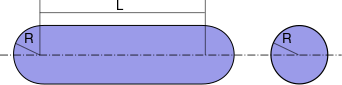
\includegraphics[width=0.7\textwidth]{gota_cilindrica.png}
  \caption{Gota cilíndrica}
  \label{fig:gotaCilindrica}
\end{figure}

\item Dos tubos de altura H, diámetro interno $d_i$ se encuentran conectados a un tanque pequeño. Los tubos y el tanque contienen agua. El sistema se encuentra unido a una plataforma, como se muestra en la figura \ref{fig:tuboU}. A qué velocidad angular $\omega$ debe girar la plataforma, de manera que la configuración de estado permanente del agua haga que ésta alcance la parte superior del tubo exterior? No tenga en cuenta los efectos de capilaridad. Exprese la solución en términos de las siquientes variables:

%% Esto son datos centrados
\begin{center}
%$\H = 16 \{cm} \d_i = 0,2 \{cm} $\\
%$\D = 8 \{cm} \h = 10 \{cm}$
$H \qquad d_i \qquad D \qquad \Delta h \qquad r$
\end{center}

%% Esto es una figura
\begin{figure}[h!!!!]
\centering
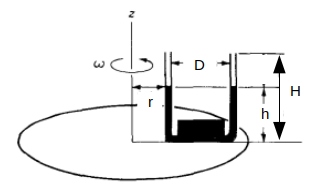
\includegraphics[width=0.5\textwidth]{tuboU.png}
\caption{Tubo en U descentrado}
\label{fig:tuboU}
\end{figure}

\clearpage
%%%Módulo 3:
%% Carga vertical y horizontal genérica de un cohete (ejemplo White 3.12, página 158, pero en vez de tiro vertical, tiro oblicuo) (C)
\item Considere un cohete con propulsión a chorro en vuelo con una inclinación $\theta$
como se muestra en la figura \ref{fig:cohete}. Utilizando balances integrales
de momento lineal, calcule la fuerza resultante sobre el cohete (considerando
también la gravedad y el efecto del chorro propulsor). Liste todas las hipótesis
utilizadas y exprese la solución en términos generales, es decir, en forma
de ecuaciones:
\begin{equation*}
F_x = F_x(\theta, \dot{m}, \vec{V}_{c}, \vec{V}_{e}, \rho)
\qquad \qquad
F_y = F_y(\theta, \dot{m}, \vec{V}_{c}, \vec{V}_{e}, \rho, \vec{g})
\end{equation*}
\\
Extienda la formulación anterior para el caso en que haya viento. Integrando la expresión que obtuvo para la fuerza, dé una expresión genérica del alcance del cohete si este parte con una inclinación $\theta_0$, con una masa de combustible $m_0$, suponiendo un flujo másico constante $\dot{m} = m_0/t_{vuelo}$.
\begin{figure}[h!!!!]
  \centering
  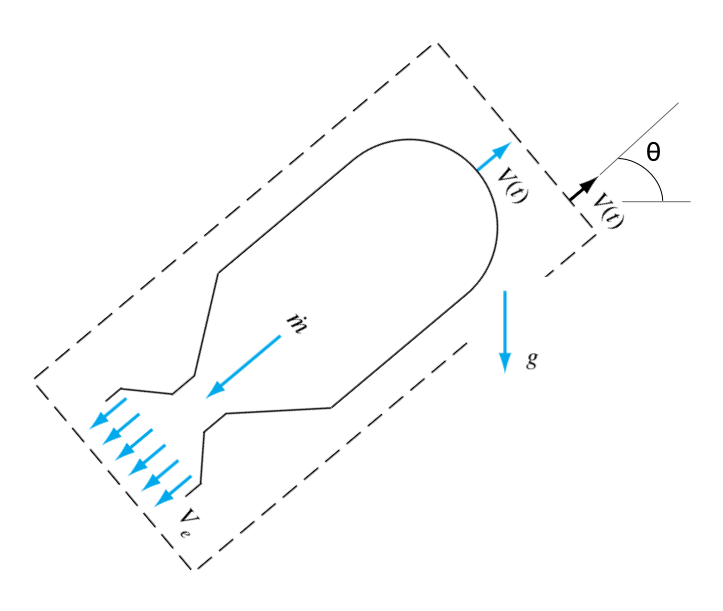
\includegraphics[width=0.7\textwidth]{rocket.png}
  \caption{Cohete en vuelo a velocidad $V(t)$ con inclinación $\theta$}
  \label{fig:cohete}
\end{figure}

\end{enumerate}

\end{document}
\noindent \underline{\textbf{Examen Final de teoría}}:

\begin{enumerate}
  \item {\bf Hidrostática}
	\begin{itemize} 
	\item Describir el principio general de la hidrostática.
	\item ¿Qué diferencias existen entre las fuerzas de superficie y de cuerpo? Dar ejemplos de cada una.
	\item Explicar mediante un ejemplo el equilibrio relativo en los casos de aceleración lineal constante y
	de rotación a velocidad constante.
	\end{itemize}
	
    \item {\bf Flujo en conductos}. Al considerar el flujo de un fluido Newtoniano en conductos cerrados.
  \begin{itemize}
  \item ¿Cuáles son las variables de interés en este problema?
  \item ¿Cuáles son los posibles regímenes de flujo?
  \item Estimativamente ¿Cuáles son los perfiles de velocidad y corte en cada caso?
  \item ¿Qué es y de qué manera pueden calcularse la pérdida de carga?
  \end{itemize}

    \item Las {\bf toberas convergentes-divergentes} son elementos de amplio uso en muchas aplicaciones de Ingeniería. El modelo matemático       empleado en su cálculo se desarrolla a partir de la teoría de flujo compresible.
    
	\begin{itemize}
	\item Definir el número de Mach y la clasificación de flujos relacionada a este coeficiente adimensional.
	\item Describir la relación entre las variaciones de presión y velocidad en función del cambio de sección.
	Analizar cómo depende del número de Mach.
	\item Describir las posibles evoluciones del flujo en la tobera convergente divergente.
	¿Qué variable determina el flujo que se desarrolla en la tobera?
	\end{itemize}
\end{enumerate}

\end{document}
%%Ejemplo de 2do examen:
\noindent\underline{\textit{Examen final de práctica}:}

\begin{enumerate}
\item El camión tanque semi remolque de la figura \ref{fig:remolque} pasa de $0$ a $7.5$ $m/s$, acelerando uniformemente durante $60s$. Se encuentra lleno de combustible ($\gamma=0,8$) \textbf{hasta la mitad} de su altura $A = 6$m. Las dimensiones restantes del contenedor son $B = 4$m y $L = 12$m. Calcular la fuerza que debe soportar la tapa trasera si la cisterna est\'a abierta y se encuentra dividida en \textbf{5 compartimientos}. A su vez, calcular qué aceleración del camión provoca el derrame de combustible.
  \begin{figure}[!ht]
    \centering
    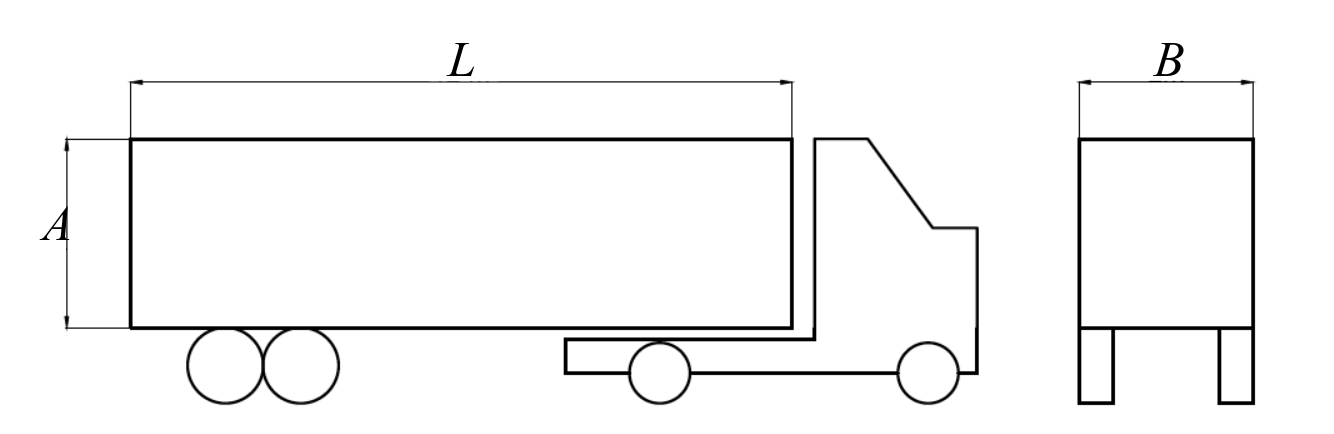
\includegraphics[width=0.8\textwidth]{camionCisterna.png}
    \caption{Esquema del camión cisterna}
    \label{fig:remolque}
  \end{figure}
  
  %% Codo 90°
\item Por el codo de la figura (\ref{fig:codo}) circulan $Q=1000 m^3/h$ de agua, con presión manométrica de entrada de $P_1 = 2 kg/cm^2$, siendo la pérdida de carga del mismo  de $\Delta h = 0.50m$. Calcular fuerza ejercida por el agua, considerando el codo emplazado en el plano horizontal. Desprecie el peso del accesorio y del agua. Los diámetros de la tubería son que $d_1=40$cm y $d_2=25$cm
  \vspace{0.5cm}
  \begin{figure}[h!!]
  \centering
   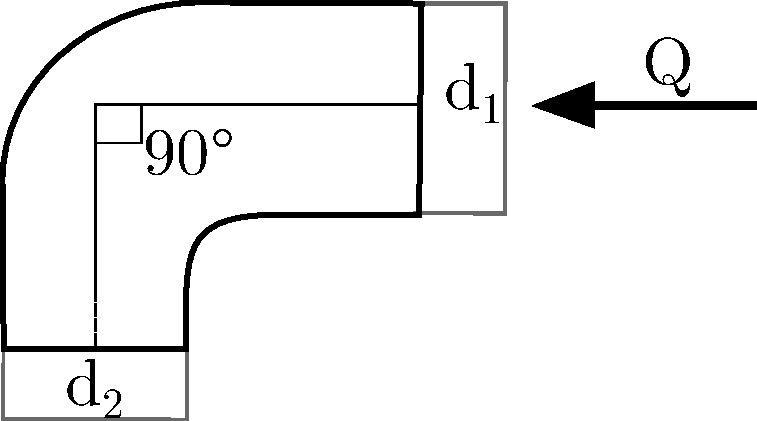
\includegraphics[width=0.5\textwidth]{codo.pdf}
  \caption{Cálculo de fuerza en codo}
  \label{fig:codo}
  \end{figure}  

\clearpage
 \item Para el circuito de la figura \ref{fig:circuito} se dispone de una bomba centrífuga con un conjunto de 4 impulsores, tal como se  muestra en la curva correspondiente de la figura \ref{fig:bomba}. Completar los siguientes items:
 \begin{enumerate}
  \item Calcular las pérdidas energéticas y trazar las líneas de energía y  gradiente hidráulico.
  \item Seleccionar, mediante la figura \ref{fig:bomba},
  el impulsor que se adecue a las demandas del sistema. En caso de ser necesario, agregar los
  accesorios que permitan alcanzar las condiciones de servicio.
  \item Calcular el valor máximo de la distancia $L_asp$ (tramo 1-2 del circuito en figura \ref{fig:circuito})  en función del ANPA requerido por la bomba (esquema figura \ref{fig:bomba}).
  \item Calcular la potencia total consumida por el equipo.
 \end{enumerate}

 \textbf{Despreciar las pérdidas localizadas.}. Fluido: agua (15 $\textordmasculine$C).
   
 Considerar el nivel de la cañería 1 coincidente con el piso (0 metros). Considerar $D_{asp} = D_1$

\begin{table}[!h]
  \centering
  \begin{tabular}{|l|c|c|p{2cm}|l|c|c|}
    \cline{1-3} \cline{5-7}
    \multicolumn{3}{|c|}{\textit{Datos}} && \multicolumn{3}{|c|}{\textit{Datos}} \\
    \cline{1-3} \cline{5-7}
    $\gamma$ & 1000 & $kg/m^3$ && $\nu$ & $10^{-6}$& $m^2/s$ \\
    \cline{1-3} \cline{5-7} 
    $p_{atm}$ & 10 & m.c.a. &&  $p_{vap}$ & 0.0176& bar \\ 
    \cline{1-3} \cline{5-7}
    $L_{asp}$ & 6 & m && $Z_{asp}$ & -3 & m \\
    \cline{1-3} \cline{5-7} 
    $L_1$ & 20 & m && $D_1$ & 0.15 & m \\ 
    \cline{1-3} \cline{5-7} 
    $L_2$ & 10 & m && $D_2$ & 0.05 & m \\ 
    \cline{1-3} \cline{5-7} 
    $L_3$ & 15 & m && $D_3$ & 0.1 & m \\ 
    \cline{1-3} \cline{5-7}
    $Z_A$ & 5 & m && $\mathbf{Q_A}$ & 30 & $m^3/h$ \\ 
    \cline{1-3} \cline{5-7}
    $Z_B$ & 10 & m && $\mathbf{Q_B}$ & 60 & $m^3/h$ \\ 
    \cline{1-3} \cline{5-7}
    $f$ & 0.022 &  && \multicolumn{2}{c|}{ANPA$_{req}$} & fig \ref{fig:bomba}\\ 
    \cline{1-3} \cline{5-7} 
  \end{tabular}  
  \caption{Datos del problema 3}
  \label{tab:circuito}
  \end{table}

\begin{figure}[hb]
\centering
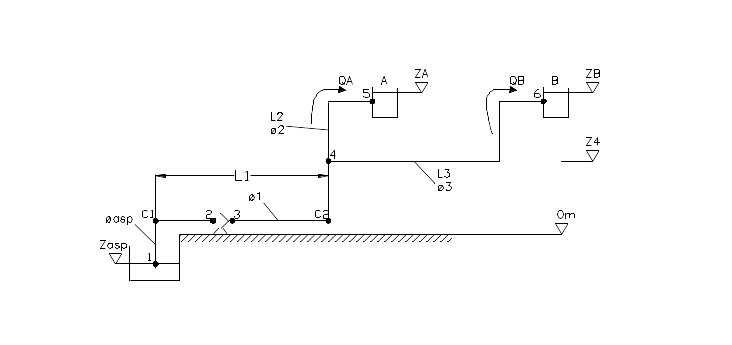
\includegraphics[width=1.1\textwidth]{circuitoGeneral.png}
\caption{Esquema del circuito}
\label{fig:circuito}
\end{figure}


\begin{figure}[hb]
\centering
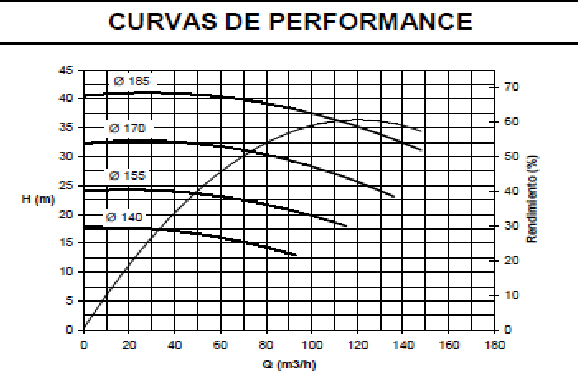
\includegraphics[width=\textwidth]{bomba.png}
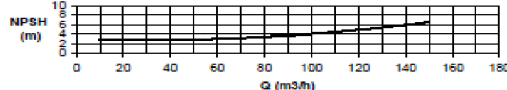
\includegraphics[width=\textwidth]{ANPA.png}
\caption{Curvas características de la bomba disponible}
\label{fig:bomba}
\end{figure}

\end{enumerate}


\end{document}
\iffalse

\MDF

\noindent\underline{\textit{Primer parcial}:} \textbf{Recuperatorio}
\begin{enumerate}
\item Las fuerzas externas pueden actuar sobre un volumen de control de dos maneras, ¿cuáles?
\item ¿En qué principio físico se basa el balance integral de energía?
%%Camion cisterna
\item El camión tanque semi remolque de la figura \ref{fig:remolque} pasa de $0$ a $15$ $m/s$, acelerando uniformemente durante $60s$. Se encuentra lleno de combustible ($\gamma=0,9$) hasta la mitad de su altura $A = 5$m. Las dimensiones restantes del contenedor son $B = 4$m y $L = 12$m. Calcular la fuerza que debe soportar la tapa trasera si la cisterna est\'a abierta y se encuentra dividida en \textbf{5 compartimientos}. A su vez, calcular qué aceleración del camión provoca el derrame de combustible.
  \begin{figure}[!ht]
    \centering
    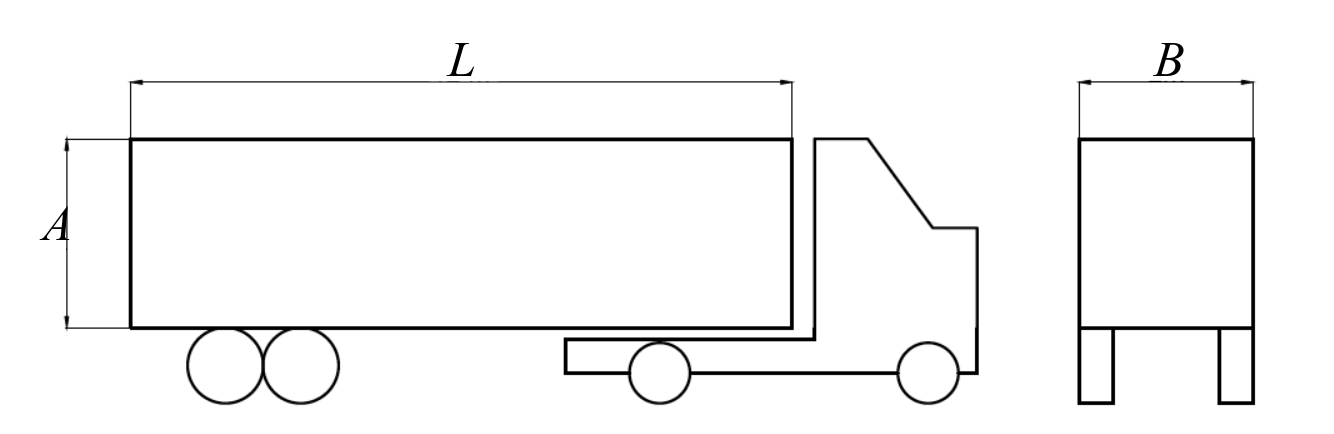
\includegraphics[width=0.8\textwidth]{camionCisterna.png}
    \caption{Esquema del camión cisterna}
    \label{fig:remolque}
  \end{figure}
  
  %% Codo 90°
\item Por el codo de la figura (\ref{fig:codo}) circulan $Q=1500 m^3/h$ de agua, con presión de entrada de \\ $P_1 = 6 kg/cm^2$, siendo la pérdida de carga del mismo  de $\Delta h = 1.0m$. Calcular fuerza ejercida por el agua, considerando el codo emplazado en el plano horizontal. Desprecie el peso del accesorio y del agua. Los diámetros de la tubería son que $d_1=30$cm y $d_2=20$cm
  \vspace{0.5cm}
  \begin{figure}[h!!]
  \centering
   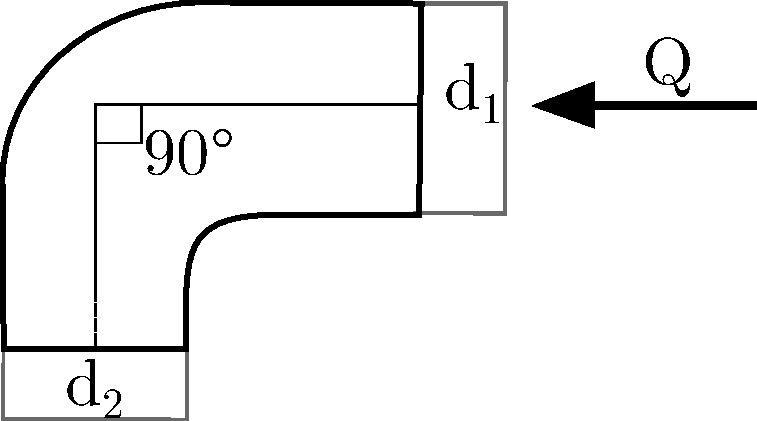
\includegraphics[width=0.5\textwidth]{codo.pdf}
  \caption{Cálculo de fuerza en codo}
  \label{fig:codo}
  \end{figure}  

\end{enumerate}
\clearpage
\fi
\MDF


\noindent\underline{\textit{Segundo parcial}: \textbf{Tema B}}
\begin{enumerate}
%% Copiar y pegar ejercicios del archivo correspondiente en la carpeta "ejercicios/"
%% Flujo Hagen Poiseuille
\item Se pretende analizar el campo de velocidades para el flujo laminar \textbf{desarrollado} en una cañería cilíndrica \textbf{infinita}, dado en la figura \ref{fig:hagen_poiseuille}. Considerando el problema \textbf{estacionario}:
\begin{enumerate}
  \item Defina las hipótesis para aplicar la ecuación de Navier-Stokes (\ref{eq:NSMom_u_cil}).
  \item Aplique simplificaciones por simetría y defina las condiciones de contorno matemáticamente.
  \item A partir de los tres apartados anteriores, obtenga la ecuación diferencial simplificada para el campo de velocidades.
  \item A partir de la solución, exprese el caudal circulante en función de los datos del problema.
\end{enumerate}

\begin{equation}\label{eq:NSMom_u_cil}
\begin{aligned}
\frac{1}{r}\frac{\partial }{\partial r} (r\,u_r)+ \frac{1}{r}\frac{\partial u_\theta}{\partial \theta} + \frac{\partial u_z}{\partial z}
&= 0 
\\
\frac{\partial u_z}{\partial t} + u_r\frac{\partial u_z}{\partial r} + \frac{u_\theta}{r}\frac{\partial u_z}{\partial \theta} + u_z \frac{\partial u_z}{\partial z}
&= -\frac{1}{\rho}\frac{\partial p}{\partial z}
+ \nu \left(\frac{1}{r}\frac{\partial}{\partial r}\left(r\frac{\partial u_z}{\partial r}\right) + \frac{1}{r^2}\frac{\partial^2 u_z}{\partial \theta^2} + \frac{\partial^2 u}{\partial z^2}\right)
\end{aligned}
\end{equation}
\begin{figure}[h!!]
\centering
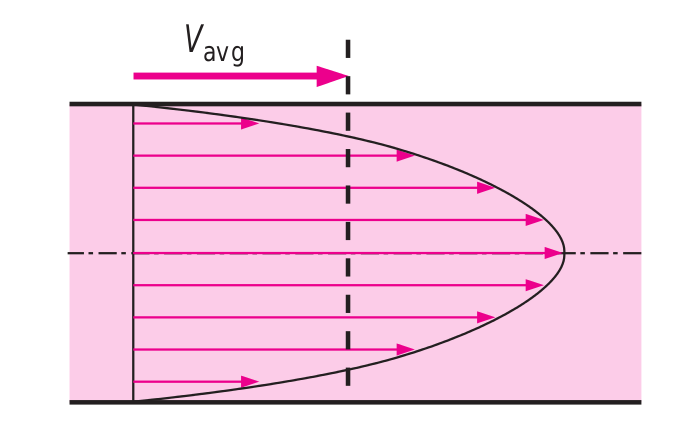
\includegraphics[width=0.4\textwidth]{hagen_poiseuille.png}
\caption{Flujo en un conducto cilíndrico}
\label{fig:hagen_poiseuille}
\end{figure}
%% Pitot en capa límite
\item La figura \ref{fig:capa_limite} muestra la ubicación de un tubo de pitot en una superficie plana que se desplaza a una velocidad $U = 5$ km/h. Utilizando la solución de capa límite de Blasius, calcular la diferencia de presión que medirá el Pitot. Recuerde que la misma corresponde a la presión dinámica del flujo $p_{din} = \rho u^2/2$. A la distancia $L$, ¿cuál es el espesor de capa límite?

Una solución aproximada a la ecuación de Blasius es el polinomio de cuarto orden dado por la ecuación \ref{eq:PolBlasius}. A continuación se listan los datos del flujo:
\begin{center}
$\rho = 1.2 kg/m^3 \qquad \mu =1.75 \times 10^{-05} Pa s\qquad L = 0.1 m \qquad h = 0.001 m$
\end{center}

\begin{equation}\label{eq:PolBlasius}
u/U = 0.0016217 \eta^4 - 0.0190921 \eta^3 + 0.0314731 \eta^2 + 0.3146989 \eta + 0.0015430 \qquad \qquad \eta = y \sqrt{\frac{U}{x\nu}}
%%  -9.2735e-05   1.5884e-03  -8.5280e-03   1.0741e-02  -8.2920e-03   3.3435e-01  -7.2436e-05 %% Mayor orden: 6
\end{equation}

\begin{figure}[h!!]
\centering
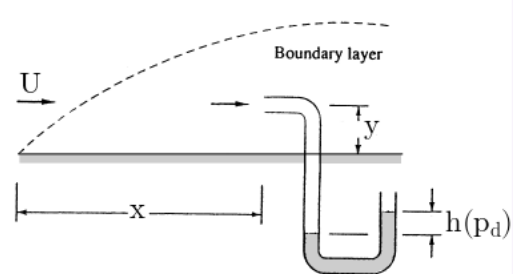
\includegraphics[width=0.4\textwidth]{capa_limite.png}
\caption{Pitot en placa plana, midiendo a una altura $h$}
\label{fig:capa_limite}
\end{figure}
\clearpage
\item Entra aire a una tobera convergente-divergente, como se muestra en la figura \ref{fig:toberaConvDiv}, a $p_0 = 2$ MPa y $T_0 = 800$ K con velocidad despreciable. El flujo es estacionario, unidimensional e isentrópico con $k = 1.4$,$R=287\;J/(kg\,K)$. Para obtener un Mach de salida $Ma_e = 3$, dada una garganta de área $A^* = 20 cm^2$, determinar:
\begin{enumerate}
\item Las condiciones de flujo en la garganta ($p_g$, $\rho_g$, $T_g$, $v_g$)
\item El flujo másico que circula por la tobera.
\item Las condiciones del flujo en el plano de la salida, inclusive el área de la salida de diseño ($A_s$, $p_s$, $\rho_s$, $T_s$, $v_s$).
\item En qué regiones de la tobera el flujo es sónico y en cuáles supersónico.
\end{enumerate}
\begin{figure}[h!!]
\centering
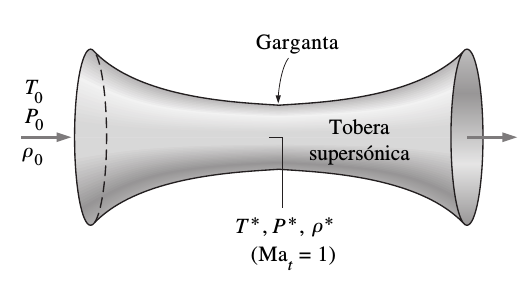
\includegraphics[width=0.5\textwidth]{toberaConvDiv.png}
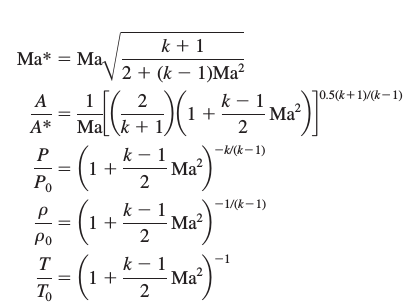
\includegraphics[width=0.5\textwidth]{eqs_comp.png}
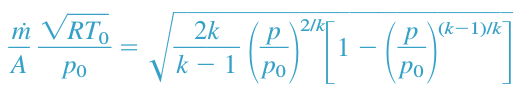
\includegraphics[width=0.5\textwidth]{mass_flux.png}
\caption{Tobera convergente divergente}
\label{fig:toberaConvDiv}
\end{figure}
\end{enumerate}

\end{document}
\clearpage
%\begin{Large}
%Todos los ejercicios
%\end{Large}
\begin{itemize}
\item Conceptos básicos 
    \begin{enumerate}
    \item ¿ La {\it "propiedad"} es una propiedad intensiva o extensiva? Analizar la pregunta para las siguientes {\it propiedades}:\\
    Volumen, masa, densidad, viscosidad, temperatura, compresibilidad, peso, deformación.
    \item ¿ La {\it "magnitud"} es una magnitud escalar, vectorial o tensorial? Analizar la pregunta para las siguientes {\it magnitudes}:\\
    Velocidad, aceleración, temperatura, esfuerzo viscoso, estado de deformación, presión.
    \item ¿ Qué tipo de sistema es un volumen de control? ¿Qué utilidad tiene en mecánica de los fluidos?
    \item ¿ En qué consiste un modelo? Dibujar un esquema donde se muestre la relación entre
    el problema físico, el problema matemático derivado y la solución obtenida.
    \item Nombrar posibles características que pueden describir un modelo de {\bf flujo}. Por otro lado, contrastarlas con las
    posibles propiedades de un {\bf fluido}.
    \item ¿Cuál es la característica principal de un flujo estacionario?
    \end{enumerate}
    
  \item Estática
    \begin{enumerate}
    \item Escribir la formulación vectorial del principio general de la hidrostática:
    \item Definición general de fuerza hidrostática sobre una superficie:
    \item Definición general de torque respecto del punto $0$ provocado por fuerza hidrostática sobre una superficie:
    \item Definir cuáles de las siguientes afirmaciones son correctas para la figura adjunta \ref{fig:hidrostat}.

      \begin{figure}[!ht]
      \centering
      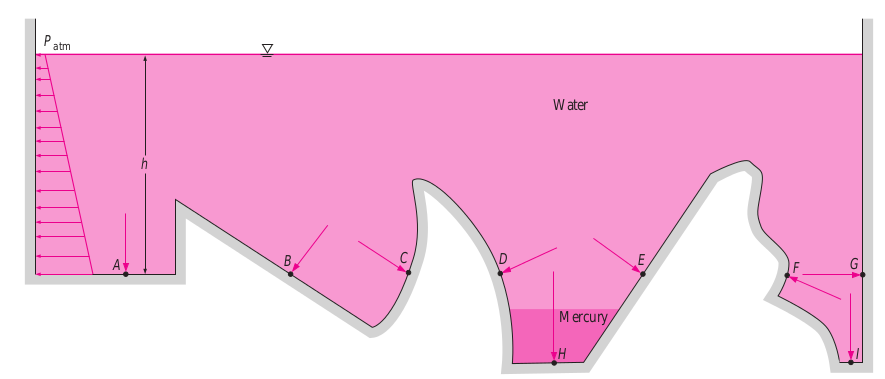
\includegraphics[width=15cm]{hidrostat.png}
      \caption{Caso hidrostática}
      \label{fig:hidrostat}
      \end{figure}

      \begin{itemize}
      \item $p_A = p_B= p_C= p_D= p_F$ \_\_\_\_
      \item $p_A = p_I$ \_\_\_\_
      \item $p_H = p_I$ \_\_\_\_
      \item $p_A = p_{atm}+\rho g h$ \_\_\_\_
      \item $\overline{F}_A = \overline{F}_B= \overline{F}_C= \overline{F}_D= \overline{F}_F$ \_\_\_\_
      \end{itemize}
      
      %   
    \item La fuerza de empuje sobre un cubo sumergido en agua sólo hasta la mitad de su altura es:

    $F_{empuje} =$ 


    \end{enumerate}
    
    \clearpage
    
   \item Cinemática
    \begin{enumerate}
    \item Dado un {\bf flujo incompresible}, escribir la ecuación de continuidad en su forma vectorial: 
    \item Escribir la derivada material desde el punto de vista Lagrangiano, Euleriano:\\
    \vskip 1.cm
    
    \item Escribir la ecuación de Bernoulli. Indicar con una cruz cuáles de las siguientes son hipótesis
    necesarias para la aplicación de dicha ecuación.

    \vskip 1.cm

      \begin{itemize}
      \item Flujo incompresible. \_\_\_\_
      \item Flujo ideal. \_\_\_\_
      \item Flujo estacionario. \_\_\_\_
      \item La única fuerza de cuerpo sobre el fluido es el peso. \_\_\_\_
      \end{itemize}

    \end{enumerate}
    
   \item Dinámica
    \begin{enumerate}
        \item Escriba la fórmula de cálculo para el número de Reynolds. $Re = $

    \end{enumerate}
    
   \item Flujos confinados
    \begin{enumerate}
    \item Escribir la fórmula de Darcy ($f$) para el cálculo de la pérdida de carga en una cañería.¿En qué unidad se obtiene el resultado?

    \vskip 1.cm

    \end{enumerate}
    
   \item Flujos compresibles
    \begin{enumerate}
    \item Escriba la fórmula de cálculo para el número de Mach. $Ma = $
    \item La velocidad de propagación del sonido ($c$) en un fluido depende de la velocidad media de flujo ($u$).
      \begin{itemize}
      \item Verdadero. \_\_\_\_
      \item Falso. \_\_\_\_
      \end{itemize}


    \end{enumerate}
    
   \item Fundamentos de máquinas hidráulicas
    \begin{enumerate}
    \item ¿Cómo se comporta la densidad de un fluido dentro de una máquina hidráulica?
    \end{enumerate}
    
   \item Bombas centrífugas
    \begin{enumerate}
    \item ¿Cuál es la principal función de una bomba hidráulica?

    \vskip 1.cm


    \end{enumerate}
    
   \item Turbinas hidráulicas
    \begin{enumerate}
    \item ¿Cuál es la principal función de una turbina hidráulica?
    \item Una turbina con número específico de revoluciones elevado es más eficiente:
		\begin{itemize}
			\item A caudales altos \_\_\_
   			\item A caudales bajos \_\_\_
		\end{itemize}    
    \end{enumerate}

    \vskip 1.cm
\end{itemize} \clearpage
\begin{itemize}
 \item {\bf Mecánica de los Fluidos:} Estática, Cinemática y Dinámica
    \begin{enumerate}
    
  \item {\bf Hidrostática}
	\begin{itemize} 
	\item Describir el principio general de la hidrostática.
	\item ¿Qué diferencias existen entre las fuerzas de superficie y de cuerpo? Dar ejemplos de cada una.
	\item Explicar mediante un ejemplo el equilibrio relativo en los casos de aceleración lineal constante y
	de rotación a velocidad constante.
	\end{itemize}


      \item La {\bf Ecuación de Bernoulli} se encuentra transcripta en \ref{eq:Bernoulli}.
	\begin{equation}\label{eq:Bernoulli}
	\frac{p}{\gamma}+	%%Energía de presión del fluido
	\frac{v^2}{2g}+	%%Energía cinética
	z=\mathit{cte} 		%%Energía potencial gravitatoria
	\end{equation}

	\begin{itemize}
	\item ¿Bajo qué hipótesis puede utilizarse este modelo matemático?
	\item ¿Qué representa cada término de la ecuación?
	\item ¿Qué representa la ecuación?¿Para qué se utiliza? Dar un ejemplo.
	\item ¿De qué forma se emplea esta ecuación en el cálculo de cañerías?
	\end{itemize}

      \item Dada la ecuación de {\bf Euler} para el momento lineal (transcripta en \ref{eq:Euler}):
      \begin{equation}\label{eq:Euler}
      \rho \frac{D\mathbf{U}}{Dt}=	%%Variación puntual de momento lineal
      \rho \mathbf{g}		%%Efecto de las fuerzas de cuerpo.
      - \nabla p 			%%Efecto de las fuerzas de presiones, fuerzas de superficie.
      \end{equation}
      \begin{itemize}
      \item ¿Bajo qué hipótesis puede utilizarse este modelo matemático?
      \item ¿Qué representa la ecuación?¿Para qué se utiliza?
      \item ¿Qué representa cada término de la ecuación?
      \item Nombrar algún ejemplo de resolución simplificada de esta ecuación.
      \end{itemize}

      Conociendo a su vez la definición de derivada material (\ref{eq:DM}),
      explicar qué tipos de aceleraciones puede experimentar una partícula
      que se desplaza en el campo de velocidad $\mathbf{U}$.

      \begin{equation}\label{eq:DM}
	\frac{Du}{DT}=\frac{\partial u}{\partial t}+u\frac{\partial u}{\partial x}+v\frac{\partial u}{\partial y}+w\frac{\partial u}{\partial z}=
	\frac{\partial u}{\partial t}+\mathbf{U}_\bullet \left(\nabla u \right)
      \end{equation}

      \item Dada la ecuación de {\bf Navier-Stokes} para el momento lineal (transcripta en \ref{eq:NS}):
      \begin{equation}\label{eq:NS}
      \rho \frac{D\mathbf{U}}{Dt}=	%%Variación puntual de momento lineal
      \rho \mathbf{g}		%%Efecto de las fuerzas de cuerpo.
      - \nabla p 			%%Efecto de las fuerzas de presiones, fuerzas de superficie.
      + \mu \nabla^2 \mathbf{U}	%%Efecto de las fuerzas viscosas, fuerzas de superficie. (de Navier-Stokes)
      \end{equation}
      \begin{itemize}
      \item ¿Bajo qué hipótesis puede utilizarse este modelo matemático?
      \item ¿Qué representa la ecuación?¿Para qué se utiliza?
      \item ¿Qué representa cada término de la ecuación?
      \item Nombrar algún ejemplo de resolución simplificada de esta ecuación.
      \end{itemize}

      Conociendo a su vez la definición de derivada material (\ref{eq:DM}),
      explicar qué tipos de aceleraciones puede experimentar una partícula
      que se desplaza en el campo de velocidad $\mathbf{U}$.

      \begin{equation}\label{eq:DM}
	\frac{Du}{DT}=\frac{\partial u}{\partial t}+u\frac{\partial u}{\partial x}+v\frac{\partial u}{\partial y}+w\frac{\partial u}{\partial z}=
	\frac{\partial u}{\partial t}+\mathbf{U}_\bullet \left(\nabla u \right)
      \end{equation}

      
      \item {\bf Teoría de capa límite}
      \begin{itemize}
      \item Explicar a qué se llama capa límite. Definir la condición de no deslizamiento.
      \item Describir los distintos tipos de capa límite posibles.
      \item ¿A qué se llama desprendimiento de capa límite? ¿En qué situación ocurre?
      \end{itemize}

      
      
      \item Las {\bf toberas convergentes-divergentes} son elementos de amplio uso en muchas aplicaciones de Ingeniería. El modelo matemático
      empleado en su cálculo se desarrolla a partir de la teoría de flujo compresible.

	\begin{itemize}
	\item Definir el número de Mach y la clasificación de flujos relacionada a este coeficiente adimensional.
	\item Describir la relación entre las variaciones de presión y velocidad en función del cambio de sección.
	Analizar cómo depende del número de Mach.
	\item Describir las posibles evoluciones del flujo en la tobera convergente divergente.
	¿Qué variable determina el flujo que se desarrolla en la tobera?
	\end{itemize}
    \end{enumerate}
	
\item {\bf Instalaciones y máquinas hidráulicas:}
    \begin{enumerate}
      \item {\bf Flujo en conductos}. Al considerar el flujo de un fluido Newtoniano
      en conductos cerrados.
      \begin{itemize}
      \item ¿Cuáles son las variables de interés en este problema?
      \item ¿Cuáles son los posibles regímenes de flujo?
      \item Estimativamente ¿Cuáles son los perfiles de velocidad y corte en cada caso?
      \item ¿Qué es y de qué manera pueden calcularse la pérdida de carga?
      \end{itemize}

      \item {\bf Turbinas}
      \begin{itemize}
      \item ¿Cuál es la principal función de dichas máquinas hidráulicas?
      \item Mencione algunos parámetros de diseño.
      \item ¿Cuáles tipos de turbinas conoce? ¿De qué depende la elección de una u otra?
      \item ¿Cuáles son las variables de contorno a las que debe ajustarse una turbina?
      \item ¿Cómo y para qué se regula el caudal que ingresa al rotor?
      \end{itemize}

      \item {\bf Bombas centrífugas}

      \begin{itemize}
      \item ¿Cuál es la principal función de dichas máquinas hidráulicas? 
	\item Explicar qué es la curva característica de la bomba y qué parámetros la afectan.
	\item ¿Cómo se interpreta el punto de trabajo?
	\item ¿Cómo se comportan dos bombas en paralelo?¿Y en serie?
      \end{itemize}

      \end{enumerate}
  \end{itemize}
\clearpage
\textbf{Primer parcial}
\begin{itemize}
%%Teoría propiedades, estática y blalances integrales
%% Propiedades y definiciones
\item ¿Cuál es la definición del concepto ``volumen de control''?
\item Las fuerzas externas pueden actuar sobre un volumen de control de dos maneras, ¿cuáles?
%% Hidrostática
\item ¿Cuál es la forma integral de la fuerza que una distribución de presiones $p(\vec{r})$ ejerce sobre una superficie $S$?
\item Escribir en forma vectorial el teorema general de la hidrostática. ¿Bajo qué hipótesis se cumple?
%% Balances integrales
\item ¿En qué principio físico se basa el balance integral de energía?
\item ¿En qué situación es nula la variación de masa dentro de un volumen de control?
%%--------------------------------------------------------
%%Ejercicios hidrostática
%%Tanques solidarios
\item Dos tanques que contienen dos fluidos diferentes se hallan separados por
una compuerta cuadrada, abisagrada en "A", como se muestra en la figura (\ref{fig:tanques}).
Cada uno de los tanques se ve sometido a una presión manométrica distinta en su
parte superior. ¿Cuál es la fuerza que debería aplicarse sobre la arista "B" para que la misma se mantenga cerrada?
\begin{center}
  $\rho_1 = 1100 \frac{kg}{m^3} \qquad P_{1,man} = -10 kPa \qquad H_1 = 10 m $\\
  $\rho_2 = 900 \frac{kg}{m^3} \qquad P_{2,man} = 50 kPa \qquad H_2 = 4 m$
\end{center}
\begin{figure}[h!!!!]
  \centering
  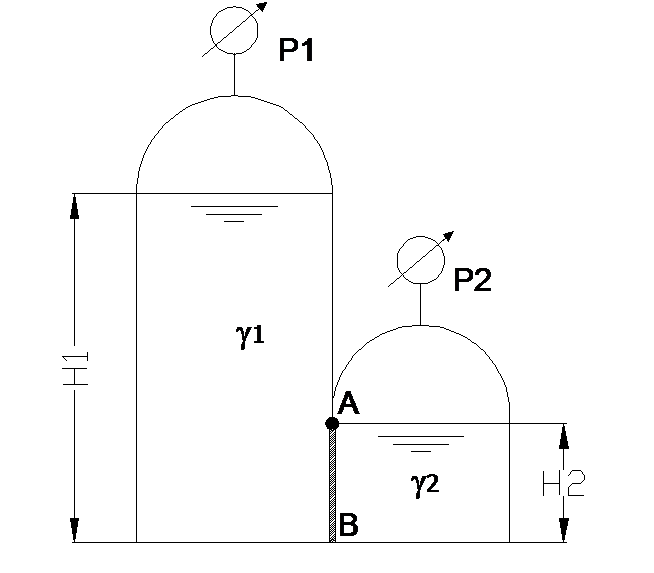
\includegraphics[width=0.4\textwidth]{tanques_solidarios.png}
  \caption{Tanques solidarios}
  \label{fig:tanques}
\end{figure}
%%Compuerta semiesférica
\item Calcular la fuerza aplicada por el fluido sobre la compuerta semiesférica representada en el esquema (\ref{fig:esfera}), sabiendo que se trata de agua a temperatura ambiente. La compuerta tiene un radio $R=1.5m$ y su  centroide se encuentra a una profundidad $H=4m$. Indique ambas componentes ($x$ e $y$) y el punto de aplicación de la fuerza.
  \begin{figure}[!!h]
    \centering
    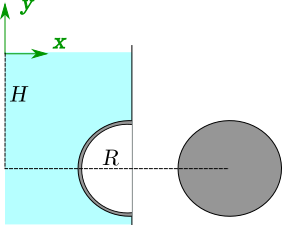
\includegraphics[width=0.4\textwidth]{compuertaEsferica.png}
    \label{fig:esfera}
    \caption{Compuerta semiesférica sumergida}
  \end{figure}

%%Camion cisterna
\item El camión tanque semi remolque de la figura \ref{fig:remolque} pasa de $0$ a $20$ $m/s$, acelerando uniformemente durante $40s$. Se encuentra lleno de combustible ($\gamma=0,8$) hasta la mitad de su altura $A = 4$m. Las dimensiones restantes del contenedor son $B = 4$m y $L = 10$m. Calcular la fuerza que debe soportar la tapa trasera si la cisterna est\'a abierta y se encuentra dividida en \textbf{5 compartimientos}. A su vez, calcular qué aceleración del camión provoca el derrame de combustible.
  \begin{figure}[!ht]
    \centering
    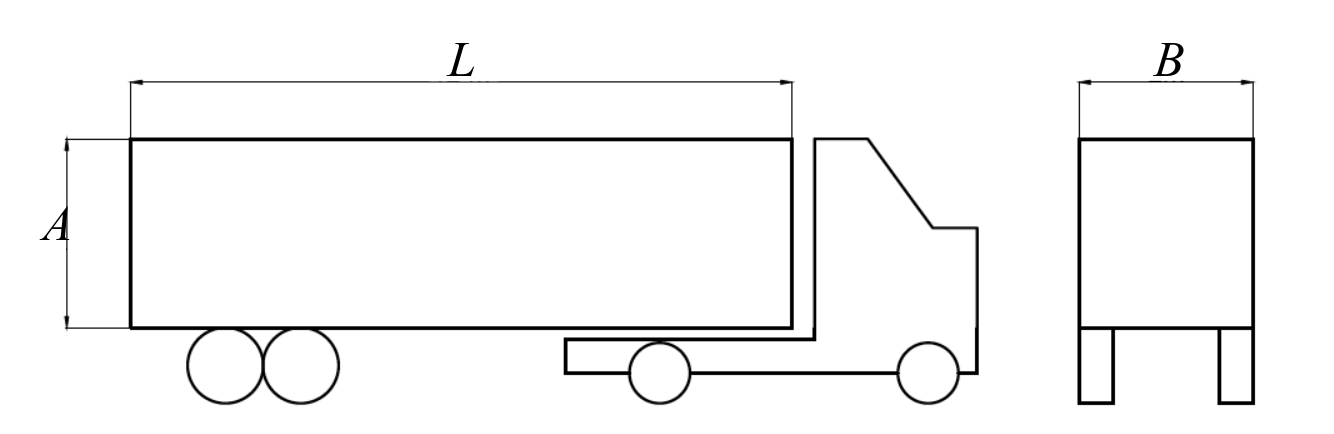
\includegraphics[width=0.8\textwidth]{camionCisterna.png}
    \caption{Esquema del camión cisterna}
    \label{fig:remolque}
  \end{figure}

%%Tanque rotante
 \item Calcular la velocidad de rotación máxima a la que puede girar el recipiente de la figura (\ref{fig:tacho}) sin que se derrame el líquido contenido en su interior. Calcular la presión sobre los puntos A y B para la velocidad de rotación calculada en el punto anterior. Los datos son los siguientes
  \begin{center}
    $\gamma = 800\frac{kgf}{m^3} \qquad H_m = 1.0 m \qquad h_0 = 0.6 m\qquad R = 0.5 m$
  \end{center}
  \begin{figure}[h!!]
    \centering
    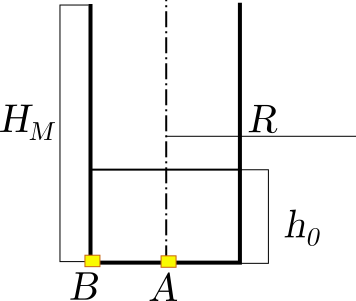
\includegraphics[width=0.4\textwidth]{tacho.png}
    \caption{Recipiente cilíndrico en rotación}
    \label{fig:tacho}
  \end{figure}

%%Ejercicios Balances integrales
%%Codo Cimbala
\item Por el codo de la figura (\ref{fig:codo}) circulan $Q=1000 m^3/h$ de agua, con presión de entrada de $P_1 = 1.5 kg/cm^2$, siendo la pérdida de carga del mismo  de $\Delta h = 1.0m$. Calcular fuerza ejercida por el agua, considerando el codo emplazado en el plano horizontal (peso en el eje y). Los diámetros de la tubería son que $d_1 = 40$cm y $d_2 = 30$cm, $\theta = 30$. 
      \vspace{0.5cm}
      \begin{figure}[h!!]
      \centering
      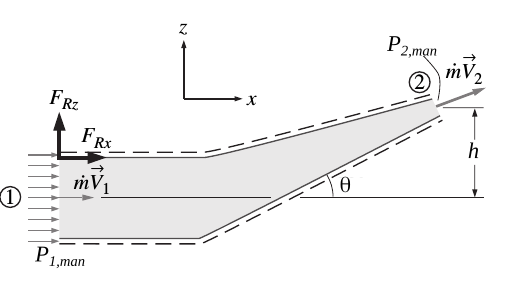
\includegraphics[width=0.5\textwidth]{codo_cimbala_gral.png}
      \caption{Cálculo de fuerza en codo}
      \label{fig:codo}
      \end{figure}  
      
      
%% Codo 90°
\item Por el codo de la figura (\ref{fig:codo}) circulan $Q=1500 m^3/h$ de agua, con presión de entrada de \\ $P_1 = 6 kg/cm^2$, siendo la pérdida de carga del mismo  de $\Delta h = 1.0m$. Calcular fuerza ejercida por el agua, considerando el codo emplazado en el plano horizontal. Desprecie el peso del accesorio y del agua. Los diámetros de la tubería son que $d_1=30$cm y $d_2=20$cm
  \vspace{0.5cm}
  \begin{figure}[h!!]
  \centering
   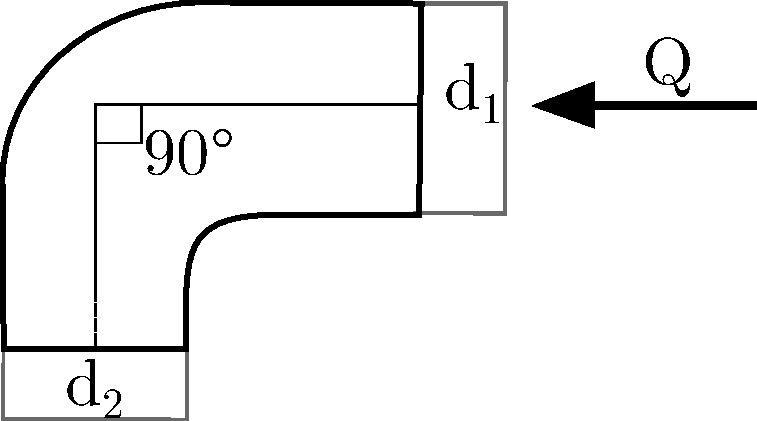
\includegraphics[width=0.5\textwidth]{codo.pdf}
  \caption{Cálculo de fuerza en codo}
  \label{fig:codo}
  \end{figure}  

%%Codo deflector móvil
\item El accesorio cuya geometría se describe en la figura (\ref{fig:codoDeflector}) se desplaza hacia la derecha con una velocidad $\vec{U} = (2.5,\;0,\;0)$m/s. Calcular la fuerza y potencia ejercida por el fluido sobre la pieza en función de los siguientes parámetros:
\begin{center}
$\rho = 1000 \frac{kg}{m^3} \qquad
\vec{V}^{abs}_1 = (8.5,\;0,\;0) \frac{m}{s} \qquad P_{1,man} = 50000 Pa
\qquad A_1 = 0.1 m^2 \qquad A_2 = 0.05 m^2$
\end{center}

\begin{figure}[h!!]
\centering
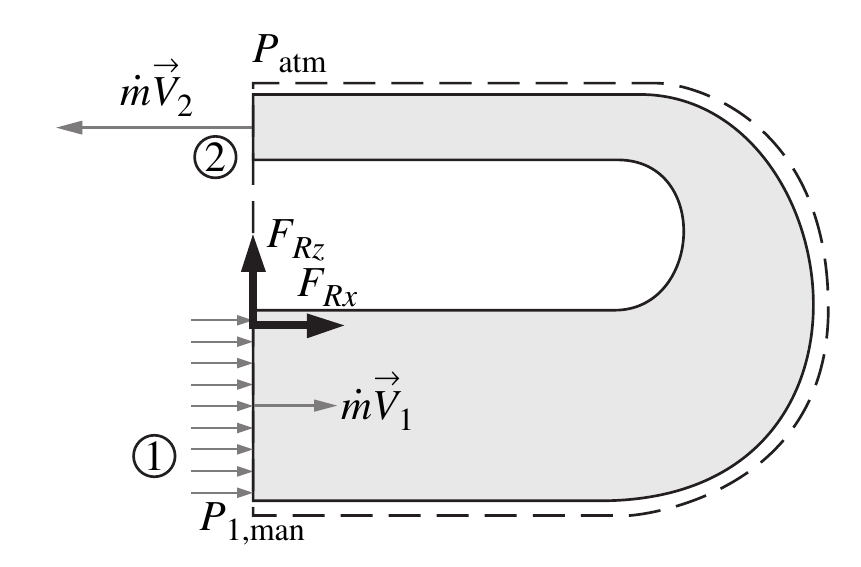
\includegraphics[width=0.4\textwidth]{codoDeflector.png}
\caption{Codo deflector, Cengel Cimbala (capítulo 6)}
\label{fig:codoDeflector}
\end{figure}

\end{itemize}
\clearpage
\textbf{Segundo parcial}
\begin{itemize}
%% Teoría blalances diferenciales (mod 4)
\item ¿Bajo qué hipótesis puede aplicarse la ecuación de flujo potencial?
\item ¿Cuál es la definición de la función linea de corriente?
\item ¿Los balances diferenciales representan conservación de propiedades en qué tipo de sistemas?
\item ¿Cuál es la diferencia entre los enfoques Euleriano y Lagrangiano?

%% Teoria flujo externo capa límite y turbulencia (mod 5)
\item Definir el concepto de capa límite. Definir la condición de no deslizamiento.
\item Escriba la fórmula de cálculo para el número de Reynolds. Dé una interpretación de dicho cociente y explique brevemente su relación con la turbulencia.
\item En aerodinámica ¿Qué es la fuerza de drag?¿Qué la produce?
\item Definir el concepto de capa límite. Definir la condición de no deslizamiento.

%% Teoría flujos compresibles (mod 6)
\item ¿Qué es el número de Mach? ¿Cómo se clasifican los flujos en función del valor del mismo?
 \item ¿De qué variables depende la velocidad del sonido en un gas ideal? ¿Qué es el número de Mach? ¿Cómo se clasifican los flujos en función del valor del mismo?
\item ¿De qué depende a velocidad de propagación del sonido en un fluido?
A la misma temperatura y presión ¿el sonido se propaga más rápido en líquidos o gases?
\item Describir las posibles evoluciones del flujo en una tobera convergente divergente. ¿Qué variables determinan el flujo que se desarrolla en la tobera?
%%-----------------------------------------------------------------------
%%Ejercicios Balances diferenciales
%Obtener ecuación de flujo Couette y Poiseuille
\item Se pretende analizar el campo de velocidades para el flujo laminar \textbf{desarrollado} entre dos placas planas \textbf{infinitas}, dado en la figura \ref{fig:placas_paralelas}. Considerando el problema \textbf{estacionario}:
\begin{enumerate}
  \item Defina las hipótesis para aplicar la ecuación de Navier-Stokes \ref{eq:NSMom_u_cart}.
  \item Defina las condiciones de contorno de este problema.
  \item Aplique las simplificaiones de simetría pertinentes.
  \item A partir de los tres apartados anteriores, obtenga la ecuación diferencial simplificada para el campo de velocidades. Explique bajo qué condiciones se obtiene flujo Poiseuille y en qué condiciones se obtiene flujo Couette.
  \item Para cada caso, grafique perfiles de velocidad y de esfuerzo de corte.
\end{enumerate}
\begin{equation}\label{eq:NSMom_u_cart}
\begin{aligned}
\frac{\partial u}{\partial x} + \frac{\partial v}{\partial y} + \frac{\partial w}{\partial z}&= 0
\\
\frac{\partial u}{\partial t} + u\frac{\partial u}{\partial x} + v\frac{\partial u}{\partial y} + w \frac{\partial u}{\partial z} = -\frac{1}{\rho}\frac{\partial p}{\partial x} + \nu \left(\frac{\partial^2 u}{\partial x^2} + \frac{\partial^2 u}{\partial y^2} + \frac{\partial^2 u}{\partial z^2}\right)
\end{aligned}
\end{equation}

\begin{figure}[h!!]
\centering
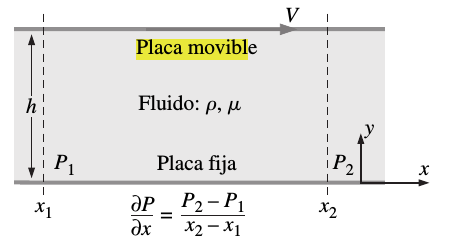
\includegraphics[width=0.6\textwidth]{placas_paralelas.png}
\caption{Flujo entre placas paralelas}
\label{fig:placas_paralelas}
\end{figure}

%% Flujo Hagen Poiseuille
\item Se pretende analizar el campo de velocidades para el flujo laminar \textbf{desarrollado} en una cañería cilíndrica \textbf{infinita}, dado en la figura \ref{fig:hagen_poiseuille}. Considerando el problema \textbf{estacionario}:
\begin{enumerate}
  \item Defina las hipótesis para aplicar la ecuación de Navier-Stokes \ref{eq:NSMom_u_cil}.
  \item Defina las condiciones de contorno de este problema.
  \item Aplique las simplificaiones de simetría pertinentes.
  \item A partir de los tres apartados anteriores, obtenga la ecuación diferencial simplificada para el campo de velocidades.
  \item A partir de la solución, exprese el caudal flujado en función de los datos del problema.
\end{enumerate}

\begin{equation}\label{eq:NSMom_u_cil}
\begin{aligned}
\frac{1}{r}\frac{\partial }{\partial r} (r\,u_r)+ \frac{1}{r}\frac{\partial u_\theta}{\partial \theta} + \frac{\partial u_z}{\partial z}
&= 0 
\\
\frac{\partial u_z}{\partial t} + u_r\frac{\partial u_z}{\partial r} + \frac{u_\theta}{r}\frac{\partial u_z}{\partial \theta} + u_z \frac{\partial u_z}{\partial z} = -\frac{1}{\rho}\frac{\partial p}{\partial z}
%+ \nu \left(\frac{1}{r}\frac{\partial}{\partial r}\left(r\frac{\partial u_z}{\partial r}\right) + \left(\frac{1}{r^2}\frac{\partial^2 u_z}{\partial \theta^2} + \frac{\partial^2 u}{\partial z^2}\right)
\end{aligned}
\end{equation}

\begin{figure}[h!!]
\centering
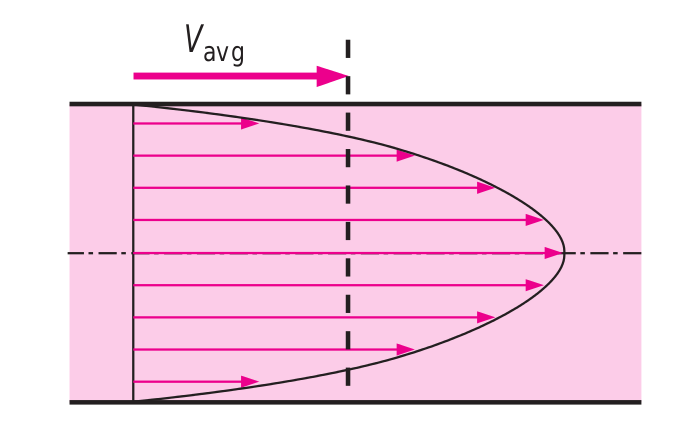
\includegraphics[width=0.6\textwidth]{hagen_poiseuille.png}
\caption{Flujo en un conducto cilíndrico}
\label{fig:hagen_poiseuille}
\end{figure}

%% Drag sobre placa plana
\item El auto de la figura \ref{fig:auto_placa} transporta una placa de madera de dimenesiones ($L = 4$m X $b =3$m) y espesor despreciable, moviéndose a una velocidad de 100 km/h. Calcule el espesor de capa límite en el extremo final de la tabla y la fuerza total de drag para régimen laminar y turbulento. ¿Cuál de los dos resultados es más preciso?
\begin{figure}[h!!]
\centering
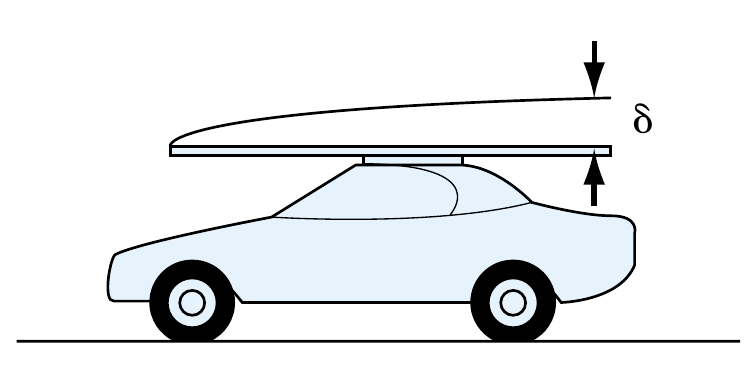
\includegraphics[width=0.4\textwidth]{auto_placa.png}
\caption{Auto transportando la placa de madera de $L$ X $b$}
\label{fig:auto_placa}
\end{figure}


%% Pitot en capa límite
\item La figura \ref{fig:capa_limite} muestra la ubicación de un tubo de pitot en una superficie plana que se desplaza a una velocidad $U = 5$ km/h. Utilizando la solución de capa límite de Blasius, calcular la diferencia de presión que medirá el Pitot. Recuerde que la misma corresponde a la presión dinámica del flujo $p_{din} = \rho u^2/2$. A la distancia $L$, ¿cuál es el espesor de capa límite?

Una solución aproximada a la ecuación de Blasius es el polinomio de cuarto orden dado por la ecuación \ref{eq:PolBlasius}. A continuación se listan los datos del flujo:
\begin{center}
$\rho = 1.2 kg/m^3 \qquad \mu =1.75 \times 10^{-05} Pa s\qquad L = 0.1 m \qquad h = 0.001 m$
\end{center}

\begin{equation}\label{eq:PolBlasius}
u/U = 0.0016217 \eta^4 - 0.0190921 \eta^3 + 0.0314731 \eta^2 + 0.3146989 \eta + 0.0015430 \qquad \qquad \eta = y \sqrt{\frac{U}{x\nu}}
%%  -9.2735e-05   1.5884e-03  -8.5280e-03   1.0741e-02  -8.2920e-03   3.3435e-01  -7.2436e-05 %% Mayor orden: 6
\end{equation}

\begin{figure}[h!!]
\centering
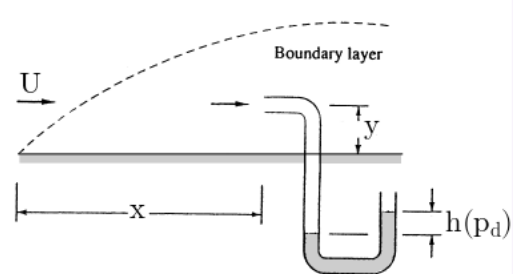
\includegraphics[width=0.4\textwidth]{capa_limite.png}
\caption{Pitot en placa plana, midiendo a una altura $h$}
\label{fig:capa_limite}
\end{figure}

%%Tobera convergente-divergente, sacado del Cimbala:
\item Entra aire a una tobera convergente-divergente, como se muestra en la figura \ref{fig:toberaConvDiv}, a $p_0$ y $T_0$ con velocidad despreciable. El flujo es estacionario, unidimensional e isentrópico con $k = 1.4$. Para obtener un Mach de salida $p_e$, dada una garganta de área $A*$, determinar:
\begin{enumerate}
\item Las condiciones de flujo en la garganta
\item Las condiciones del flujo en el plano de la salida, inclusive el área de la salida de diseño ($Ma_e$, $v_e$, $T_e$).
\item El flujo másico que circula por la tobera.
\item En qué regiones el flujo es sónico y en cuáles supersónico.
\end{enumerate}
\begin{figure}[h!!]
\centering
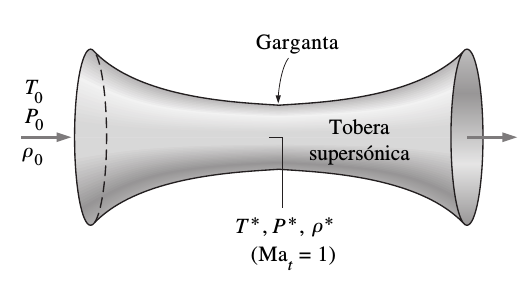
\includegraphics[width=0.5\textwidth]{toberaConvDiv.png}
%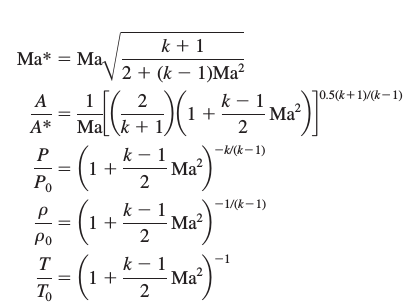
\includegraphics[width=0.5\textwidth]{eqs_comp.png}
\caption{Tobera convergente divergente}
\label{fig:toberaConvDiv}
\end{figure}
\begin{equation*}
\begin{aligned}
\frac{A}{A^*} = \frac{1}{\text{Ma}}\left[\left(\frac{2}{k+1}\right) \left(1 + \frac{k-1}{2}\text{Ma}^2\right)\right]^{0.5(k+1)/(k-1)}
\qquad
\frac{T}{T_0} = \left(1 + \frac{k-1}{2}\text{Ma}^2\right)^{-1}
\\
\frac{p}{p_0} = \left(1 + \frac{k-1}{2}\text{Ma}^2\right)^{-k/(k-1)}
\qquad
\frac{\rho}{\rho_0} = \left(1 + \frac{k-1}{2}\text{Ma}^2 \right)^{-1/(k-1)}
\end{aligned}
\end{equation*}


\end{itemize}
\clearpage
\textbf{Tercer parcial}
\begin{itemize}
%%Teoría flujo interno (mod 7)
 \item Explicar la vinculación entre las pérdidas de carga y los caudales en los casos en donde dos cañerías trabajan en paralelo.


%%Teoría máquinas hidráulicas (mod 8)
 \item ¿Cuál es la principal función de una bomba hidráulica?¿De qué parámetros de diseño depende su curva característica?
 \item ¿Cual es la principal función de una turbina hidráulica? ¿Qué es y para qué sirve el número específico de revoluciones?
 \item ¿Qué es y cómo se interpreta el punto de trabajo de una bomba en un sistema de cañerías?

%%Teoría Intro CFD (mod 9)




%%---------------------------------------------------------------------------



%% Ejercicios bombas e instalaciones
 \item Para el circuito de la figura \ref{fig:circuito} se dispone de una bomba centrífuga con un conjunto de 4 impulsores, tal como se  muestra en la curva correspondiente de la figura \ref{fig:bomba}. Completar los siguientes items:
 \begin{enumerate}
  \item Calcular las pérdidas energéticas y trazar las líneas de energía y  gradiente hidráulico.
  \item Seleccionar, mediante la figura \ref{fig:bomba},
  el impulsor que se adecue a las demandas del sistema. En caso de ser necesario, agregar los
  accesorios que permitan alcanzar las condiciones de servicio.
  \item Calcular el valor máximo de la distancia $L_asp$ (tramo 1-2 del circuito en figura \ref{fig:circuito})  en función del ANPA requerido por la bomba (esquema figura \ref{fig:ANPA}).
  \item Calcular la potencia total consumida por el equipo.
 \end{enumerate}

 \textbf{Despreciar las pérdidas localizadas.}. Fluido: agua (15 $\textordmasculine$C).
   
 Considerar el nivel de la cañería 1 coincidente con el piso (0 metros).

\begin{table}[!h]
  \centering
  \begin{tabular}{|l|c|c|p{2cm}|l|c|c|}
    \cline{1-3} \cline{5-7}
    \multicolumn{3}{|c|}{\textit{Datos}} && \multicolumn{3}{|c|}{\textit{Datos}} \\
    \cline{1-3} \cline{5-7}
    $\gamma$ & 1000 & $kg/m^3$ && $\nu$ & $10^{-6}$& $m^2/s$ \\
    \cline{1-3} \cline{5-7} 
    $p_{atm}$ & 10 & m.c.a. &&  $p_{vap}$ & 0.0176& bar \\ 
    \cline{1-3} \cline{5-7}
    $L_{asp}$ & 6 & m && $Z_{asp}$ & -2 & m \\
    \cline{1-3} \cline{5-7} 
    $L_1$ & 20 & m && $D_1$ & 0.15 & m \\ 
    \cline{1-3} \cline{5-7} 
    $L_2$ & 10 & m && $D_2$ & 0.04 & m \\ 
    \cline{1-3} \cline{5-7} 
    $L_3$ & 15 & m && $D_3$ & 0.05 & m \\ 
    \cline{1-3} \cline{5-7}
    $Z_A$ & 8 & m && $\mathbf{Q_A}$ & 40 & $m^3/h$ \\ 
    \cline{1-3} \cline{5-7}
    $Z_B$ & 8 & m && $\mathbf{Q_B}$ & 60 & $m^3/h$ \\ 
    \cline{1-3} \cline{5-7}
    $f$ & 0.022 &  && \multicolumn{2}{c|}{ANPA$_{req}$} & fig \ref{fig:ANPA}\\ 
    \cline{1-3} \cline{5-7} 
  \end{tabular}  
  \caption{Datos del problema 3}
  \label{tab:circuito}
  \end{table}

\begin{figure}[hb]
\centering
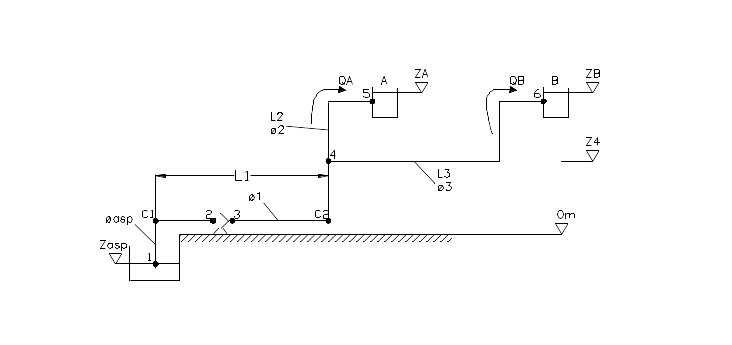
\includegraphics[width=0.8\textwidth]{circuitoGeneral.png}
\caption{Esquema del circuito}
\label{fig:circuito_gen}
\end{figure}


\begin{figure}[hb]
\centering
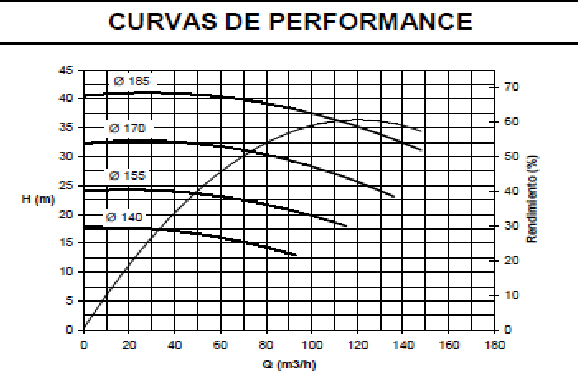
\includegraphics[width=\textwidth]{bomba.png}
\caption{Curvas características de la bomba disponible}
\label{fig:bomba}
\end{figure}

\begin{figure}[hb]
\centering
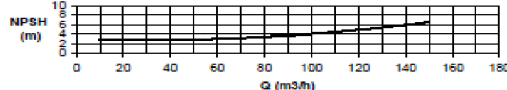
\includegraphics[width=\textwidth]{ANPA.png}
\caption{ANPA requerido por la bomba}
\label{fig:ANPA}
\end{figure}

%% 
 \item En el sistema de la figura (\ref{fig:circuito}) se deben cumplir las condiciones indicadas. Se dispone de dos bombas centrífugas idénticas, una instalada en el sistema y otra disponible para su uso en caso de ser necesario. Las características de las bombas  se detallan en la tabla.
 \begin{enumerate}
  \item Verificar si la bomba instalada cumple con las condiciones de servicio. En caso de no ser así, proponer soluciones.
  \item Calcular, de ser necesario, la pérdida de carga que debería generar una válvula para garantizar la distribución de caudales requerida por diseño.
%   \item Calcular la potencia que debe suministrar el motor a la bomba ($\eta_{mec}=0.92$)
 \end{enumerate}
 Considerar a su vez los siguientes datos:
 \begin{itemize}
  \item La velocidad de operación de la bomba es $n=1500RPM$.
  \item El fluido impulsado es agua ($\gamma = 1000 kgf/m^3$ y $\nu = 1 \times 10^{-6}m/s^2$).
  \item Las pérdidas locales son despreciables.
  \item El factor de Darcy de todas las cañerías puede aproximarse como $f=0.02$.
  \end{itemize}
  \vspace{-1cm}
\begin{figure}[!!!ht]
  \centering
   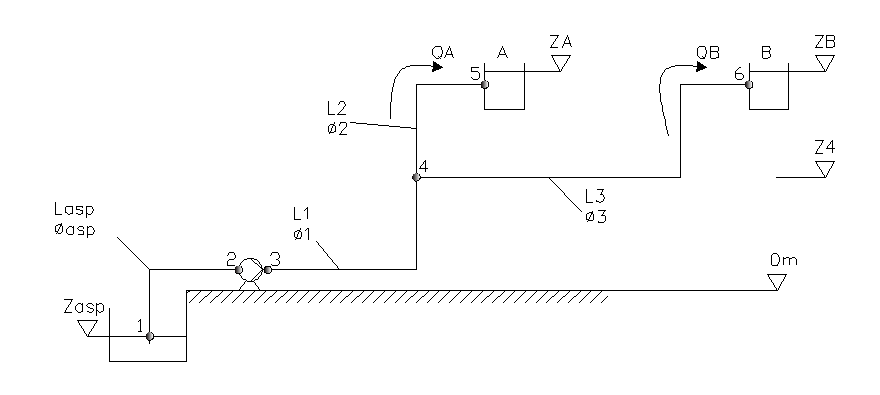
\includegraphics[width=14cm]{circuito.png}
  \caption{Esquema del circuito indicado}
  \label{fig:circuito}
  \end{figure}

  \begin{table}[!h]
  \centering
  \begin{tabular}{|l|c|c|c|c|r|}
    \hline 
    {\bf Q} & 100 & 150 & 350 & 500 & [$l/s$] \\ 
    \hline 
    {\bf H} & 98 & 95 & 93 & 89 & [$m$] \\ 
    \hline 
    $ANPA_{req}$ & 1.3 & 2.2 & 2.6 & 2.9 & [$m$] \\ 
    \hline 
  \end{tabular}  
  \caption{Propiedades de las bombas disponibles}
  \label{tab:bomba}
  \end{table}

\end{itemize}\clearpage


\end{document}

%%Ejemplo primer parcial
\MDF
\underline{\textit{Primer parcial}: \textbf{Tema A}}

\begin{enumerate}
      \item ¿Cuál es la definición del concepto ``volumen de control''?
      \item Escribir en forma vectorial el teorema general de la hidrostática. ¿Bajo qué hipótesis se cumple?
      \item ¿En qué principio físico se basa el balance integral de energía?
      \item Dos tanques que contienen dos fluidos diferentes se hallan separados por
      una compuerta cuadrada, abisagrada en "A", como se muestra en la figura (\ref{fig:tanques}).
      Cada uno de los tanques se ve sometido a una presión manométrica distinta en su
      parte superior. ¿Cuál es la fuerza que debería aplicarse sobre la arista "B" para que la misma se mantenga cerrada?
      \begin{center}
    $\rho_1 = 1100 \frac{kg}{m^3} \qquad P_{1,man} = -10 kPa \qquad H_1 = 10 m $\\
    $\rho_2 = 900 \frac{kg}{m^3} \qquad P_{2,man} = 50 kPa \qquad H_2 = 4 m$
    \end{center}
      \begin{figure}[!ht]
	\centering
	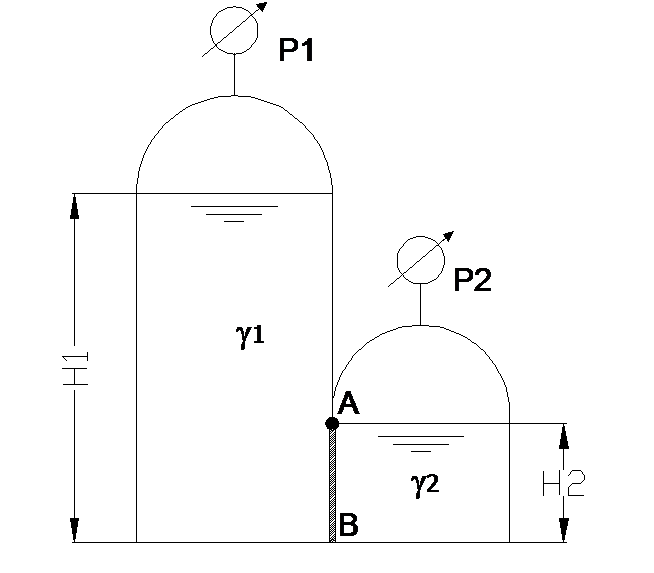
\includegraphics[width=0.4\textwidth]{tanques_solidarios.png}
	\caption{Tanques solidarios}
	\label{fig:tanques}
	\end{figure}
      \item Por el codo de la figura (\ref{fig:codo}) circulan $Q=1000 m^3/h$ de agua, con presión de entrada de $P_1 = 1.5 kg/cm^2$, siendo la pérdida de carga del mismo  de $\Delta h = 1.0m$. Calcular fuerza ejercida por el agua, considerando el codo emplazado en el plano horizontal (peso en el eje y). Los diámetros de la tubería son que $d_1 = 40$cm y $d_2 = 30$cm. 
      \vspace{0.5cm}
      \begin{figure}[!ht]
      \centering
      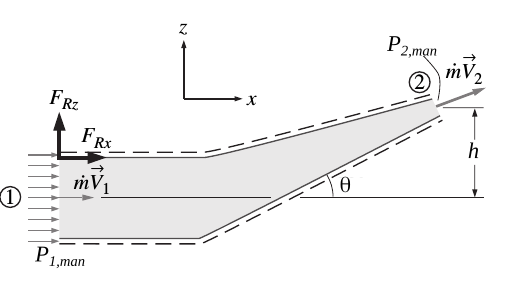
\includegraphics[width=0.5\textwidth]{codo_cimbala_gral.png}
      \caption{Cálculo de fuerza en codo}
      \label{fig:codo}
      \end{figure}  
\end{enumerate}
\clearpage

\MDF

\underline{\textit{Primer parcial}: \textbf{Tema B}}

\begin{enumerate}
  \item Las fuerzas externas pueden actuar sobre un volumen de control de dos maneras, ¿cuáles?
  \item ¿Cuál es la forma integral de la fuerza que una distribución de presiones $p(\vec{r})$ ejerce sobre una superficie $S$?
  \item ¿En qué situación es nula la variación de masa dentro de un volumen de control?
  \item El camión tanque semi remolque de la figura \ref{fig:remolque} pasa de $0$ a $20$ $m/s$, acelerando uniformemente durante $40s$. Se encuentra lleno de combustible ($\gamma=0,8$) hasta la mitad de su altura $A = 4$m. Las dimensiones restantes del contenedor son $B = 4$m y $L = 10$m. Calcular la fuerza que debe soportar la tapa trasera si la cisterna est\'a abierta y se encuentra dividida en \textbf{5 compartimientos}. A su vez, calcular qué aceleración del camión provoca el derrame de combustible.
  \begin{figure}[!ht]
    \centering
    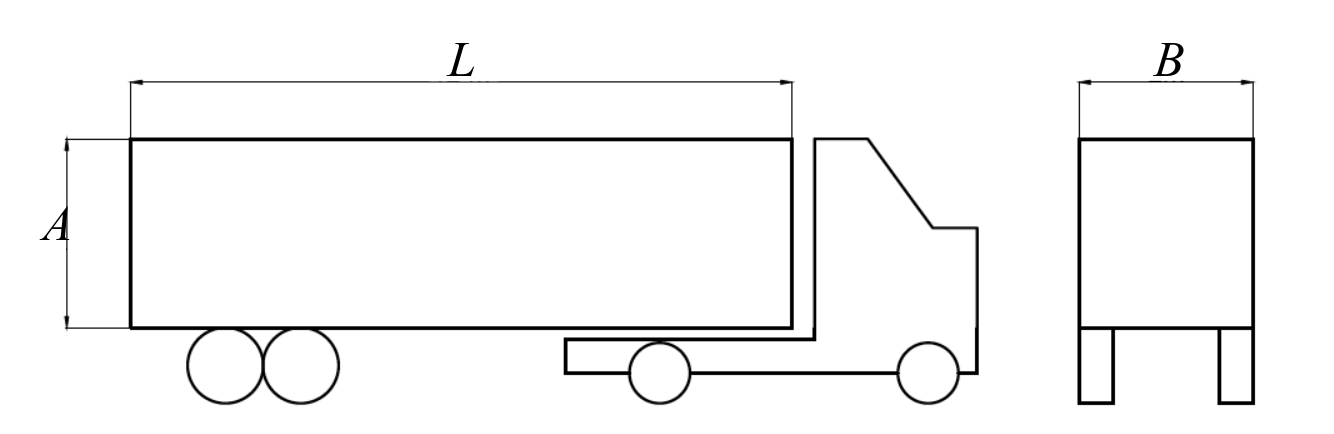
\includegraphics[width=0.8\textwidth]{camionCisterna.png}
    \caption{Esquema del camión cisterna}
    \label{fig:remolque}
  \end{figure}
  \item El accesorio cuya geometría se describe en la figura (\ref{fig:codoDeflector}) se desplaza hacia la derecha con una velocidad $\vec{U} = (5,\;0,\;0)$m/s. Calcular la fuerza en el sentido $x$ y la potencia ejercida por el fluido sobre la pieza en función de los siguientes parámetros:
    \begin{center}
    $\rho = 1000 \frac{kg}{m^3} \qquad
    \vec{V}^{abs}_1 = (10,\;0,\;0) \frac{m}{s} \qquad P_{1,man} = 10000 Pa$
    \vspace{0.25cm}
    $A_1 = 0.1 m^2 \qquad A_2 = 0.05 m^2$
    \end{center}
      \begin{figure}[hb]
    \centering
    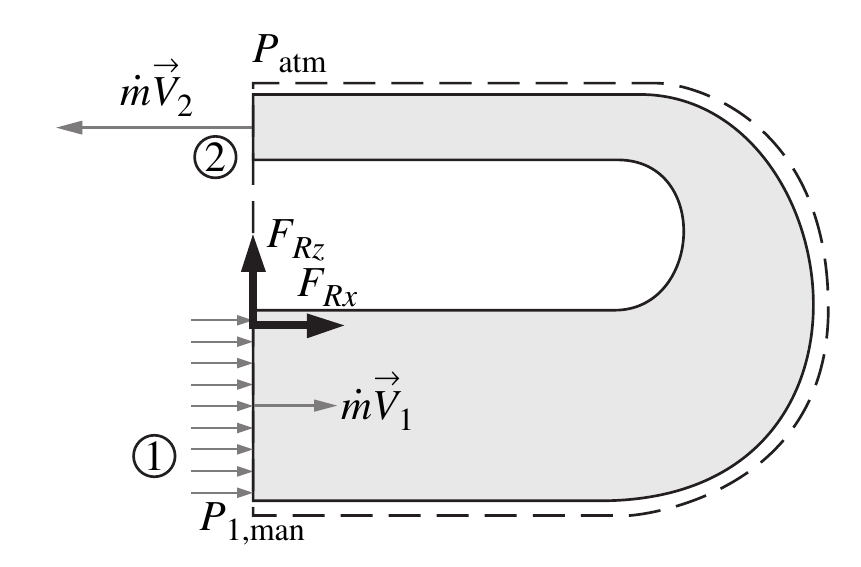
\includegraphics[width=0.45\textwidth]{codoDeflector.png}
    \caption{Codo deflector, extraído del capítulo 6 del Cengel Cimbala}
    \label{fig:codoDeflector}
    \end{figure}
  \end{enumerate}
